%
%                           	Portada
%
%           Contiene los comandos necesarios para generar la portada
%                			  del documento
%
%-------------------------------------------------------------------------
%
%Copyright 2020 David Torrez Reyes
%This file is part of BookTemplate.
%
%BookTemplate is free software: you can redistribute it and/or modify
%it under the terms of the GNU General Public License as published by
%the Free Software Foundation, either version 3 of the License, or
%(at your option) any later version.
%
%BookTemplate is distributed in the hope that it will be useful,
%but WITHOUT ANY WARRANTY; without even the implied warranty of
%MERCHANTABILITY or FITNESS FOR A PARTICULAR PURPOSE.  See the
%GNU General Public License for more details.
%
%You should have received a copy of the GNU General Public License
%along with BookTemplete.  If not, see <https://www.gnu.org/licenses/>.
%-------------------------------------------------------------------------


%----------------------------------------------
%				Primera portada
%----------------------------------------------

% Estilo de pagina vacío, No genera encabezado
\thispagestyle{plain}
\pagenumbering{Roman}

% Creamos el entorno para generar portada
\begin{titlepage}
	\centering
	% Genera una linea de la longitud del texto con grosor de 1.5 pts
	\rule{\textwidth}{1.5pt} 
		% Cambio tamaño de letra grande (\huge) y texto en negritas
		% Llamamos a la constante \titulo
		{\huge\bfseries		\titulo 	\par}
	% Genera una linea de la longitud del texto con grosor de 1.5 pts
	\rule{\textwidth}{1.5pt} \par
	% Dejamos un espacio de 3cm
	\vspace{3cm}
		% Llamamos a la constante \autor y cambiamos el tamaño de letra a (Large)
		{\huge	\autor \par}
	% Deja un espacio de 3cm
	\vspace{3cm}	
		%Incluimos una imagen de portada
		{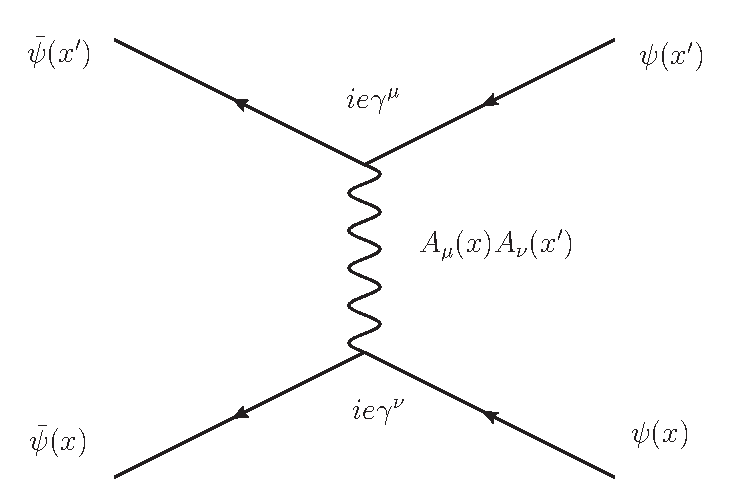
\includegraphics{diagrama_portada} \par}
		% Dejamos un espacio de 2.5cm
	\vspace{2.5cm}
		% Generamos la fecha
		{\huge	\today \par}
		% Genera una linea de la longitud del texto con grosor de 1.5 pts
	\rule{\textwidth}{1.5pt}
\end{titlepage}

%----------------------------------------------
%				Segunda portada
%----------------------------------------------

% Estilo de pagina vacío, No genera encabezado
\thispagestyle{empty}
% Creamos el entorno para generar portada
\begin{titlepage}
	\centering
	\vspace{10cm}
	% Genera una linea de la longitud del texto con grosor de 1.5 pts
	\rule{\textwidth}{1.5pt} 
		% Cambio tamaño de letra grande (\huge) y texto en negritas
		% Llamamos a la constante \titulo
		{\huge\bfseries		\titulo 	\par}
	% Genera una linea de la longitud del texto con grosor de 1.5 pts
	\rule{\textwidth}{1.5pt}
	% Termina el párrafo del titulo
	\par
	% Deja un espacio de 5cm
	\vspace{5cm}	
		{\huge Notas de Teoría Cuántica de Campos \par}
	% Deja un espacio de 5cm
	\vspace{4cm}
	% Llamamos a la constante \autor y cambiamos el tamaño de letra a (Large)
		{\huge	\autor \par}
	% Dejamos un espacio de 3cm
	\vspace{4cm}
		% Generamos la fecha
		{\Large	\today \par}
	\vspace{3cm}
		% Copyright
		{\Large \copyright{} Copyright  2020  \autor}

	\end{titlepage}

